% File:  /mit/8.13/presentations/zipped-sample-presentation/sample-presentation.tex
% Updated: June 11, 2008
% Summary: LaTeX template for creating Junior Lab presentations.
%
% Usage: To build a PDF, type `pdflatex sample-presentation.tex'
%        THREE TIMES in order to correct all internal references.
% The Beamer Package Users Guide can be viewed at
% /mit/8.13/presentations/beamerusersguide.pdf
% The users guide is a 224 page document so please don't print it out!

\documentclass[hyperref=pdftex, presentation]{beamer}
% Replacing 'presentation' with 'handout' in the above line
% will produce 4 slides per page.
% The hyperref option makes it possible to include hyperlinks.

\mode<presentation> {
  \usetheme{Boadilla}
  % or CambridgeUS, boxes, Warsaw, Madrid, many others
   \setbeamercovered{transparent}
  % or whatever (possibly just delete it)
  }

\usepackage[english]{babel}
\usepackage[latin1]{inputenc}
\usepackage{times}
\usepackage[T1]{fontenc}
% Or whatever. Note that the encoding and the font should match. If T1
% does not look nice, try deleting the line with the fontenc.

\mode<handout>{
\usepackage{pgfpages}
\pgfpagesuselayout{4 on 1}[a4paper,landscape,border shrink=5mm]
\setbeamercolor{background canvas}{bg=black!10} }

%%%%%%%%%%%%%%%%%%%%%%%%%%%%%%%%%%%%%%%%%%%%%%%%%%%%%%%%%%%%%%%%%%%%%%

\title[Measuring Planck's Constant] % (optional)
{Measuring Planck's Constant Within the Framework of the Photoelectric Effect}

% \subtitle
% {Presentation Subtitle} % (optional)

\author[Octavio Vega]{Octavio Vega}
\institute[] {MIT - Department of Physics\\}
\date[\today]


% If you wish to uncover everything in a step-wise fashion, uncomment
% the following command:

% \beamerdefaultoverlayspecification{<+->}

% If you wish to uncover everything step by step step just add the command \pause on the specific place.
% Several places are suggested. Just uncomment \pause commands.
% Also- on Organization of talk  [pausesections] as an option.
% Adding the option [handout] to the \documentclass definition will automatically disable all \pause commands
% and will make the frame into slides- in nice printable format.

%;;;;;;;;;;;;;;;;;;;;;;;;;;;;;;;;;;;;;;;;;;;;;;;;;;;;;;;;;;;;;;;;;;;;;;;;;;;;;;;;;;;;;
\begin{document}
\begin{frame}
  \titlepage
\end{frame}



%;;;;;;;;;;;;;;;;;;;;;;;;;;;;;;;;;;;;;;;;;;;;;;;;;;;;;;;;;;;;;;;;;;;;;;;;;;;;;;;;;;;;;

%columns & blocks: There are two handy environments for structuring
%your slide: "blocks", which divide your slide (horizontally) into
%headed sections, and "columns" which divides your slide (vertically)
%into colum%ns.  This next frame demonstrates both.

\begin{frame}{\Large The Roots of the Photoelectric Effect}
\begin{columns}[c] % the "c" option specifies center vertical
           % alignment, a `t' option would align the contents
           % top vertically

\column{.7\textwidth} % column designated by a command
\begin{block}{Origins}
\begin{itemize}
 \item In 1887 Heinrich Hertz discovered the photoelectric effect.
 \item Motivated by the UV light from sparks of his radio wave generator causing electric current to flow between the electrodes of the generator. 
\end{itemize}
\end{block}
\begin{block}{Advancements}
\begin{itemize}
 \item Meanwhile, Philip Leonard concluded that charge-to-mass ratio of emitted charge was identical to the electrons which had already been discovered by J.J. Thomson.
 \item Albert Einstein later officially linked the idea of quantized emissions with the photoelectric effect
\end{itemize}
\end{block}
\column{.3\textwidth}

\end{columns}
\end{frame}


%;;;;;;;;;;;;;;;;;;;;;;;;;;;;;;;;;;;;;;;;;;;;;;;;;;;;;;;;;;;;;;;;;;;;;;;;;;;;;;;;;;;;;
\begin{frame}{Particle-Wave Duality and the Motivation for Photocurrent}
 \small
 \begin{itemize}
  \item In 1900, Max Planck proposed crucial idea that matter radiates energy in "packets" or \textit{quanta} of energy given by $h\nu$
  \item Idea: demonstrate this by having beams of light incident on a metal surface eject electrons
  \item Remaining kinetic energy of electron after being ejected given by
   $K=h\nu-\phi$
    \begin{itemize}
    	\item $\nu$ is the frequency of incident light,
    	\item $\phi$ is the work function of the material; represents binding energy holding electron,
    	\item $h$ is Planck's constant-- our constant of interest.
    \end{itemize}
\item An opposing electric field, generated by a retarding voltage, may hinder the photoelectrons. We define a stopping voltage V to be such that the induced electric field stops photocurrent:
$$eV=K=h\nu-\phi=0$$ where $e$ is the electron charge ($1.6\cdot10^{-19}$ Coulombs)
 \end{itemize}
\end{frame}

%;;;;;;;;;;;;;;;;;;;;;;;;;;;;;;;;;;;;;;;;;;;;;;;;;;;;;;;;;;;;;;;;;;;;;;;;;;;;;;;;;;;;;
\begin{frame}{\Large Cutoff Voltages and Detecting Photocurrent}

 \parbox{4in}{
 \begin{itemize}
  \item Solving above equation for stopping voltage gives
     $V_{\mathrm{stop}} = \frac{h}{e}\nu -\frac{\phi}{e}$
  \item The above relation relates $V_{\mathrm{stop}}$ to incident frequencies. 
 \end{itemize}
 }%
 ~~~~%

\begin{figure}
 \centering
 \parbox{4cm}{
 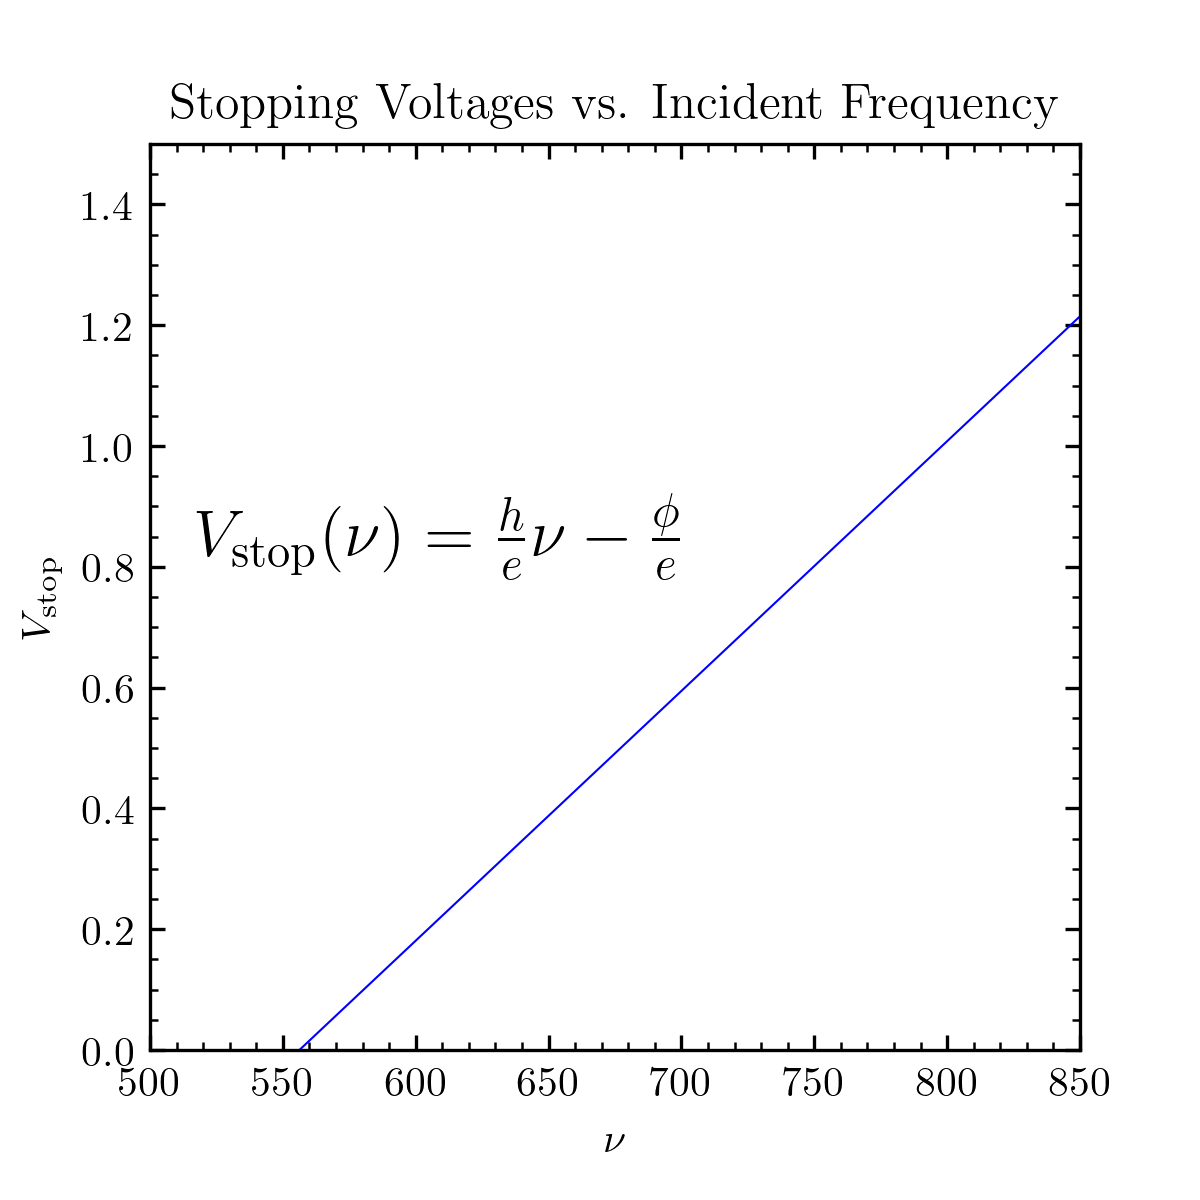
\includegraphics[width=4cm]{sample_stopping_volts.png}
 }
 \caption{A sample theoretical plot of stopping voltage over frequencies.}
\end{figure}
%\pause

We will investigate this linear relationship with different frequencies and stopping voltages to find an estimate for Planck's constant. 

\end{frame}




%;;;;;;;;;;;;;;;;;;;;;;;;;;;;;;;;;;;;;;;;;;;;;;;;;;;;;;;;;;;;;;;;;;;;;;;;;;;;;;;;;;;;;
\begin{frame}{Apparatus}
\begin{figure}
	\centering
	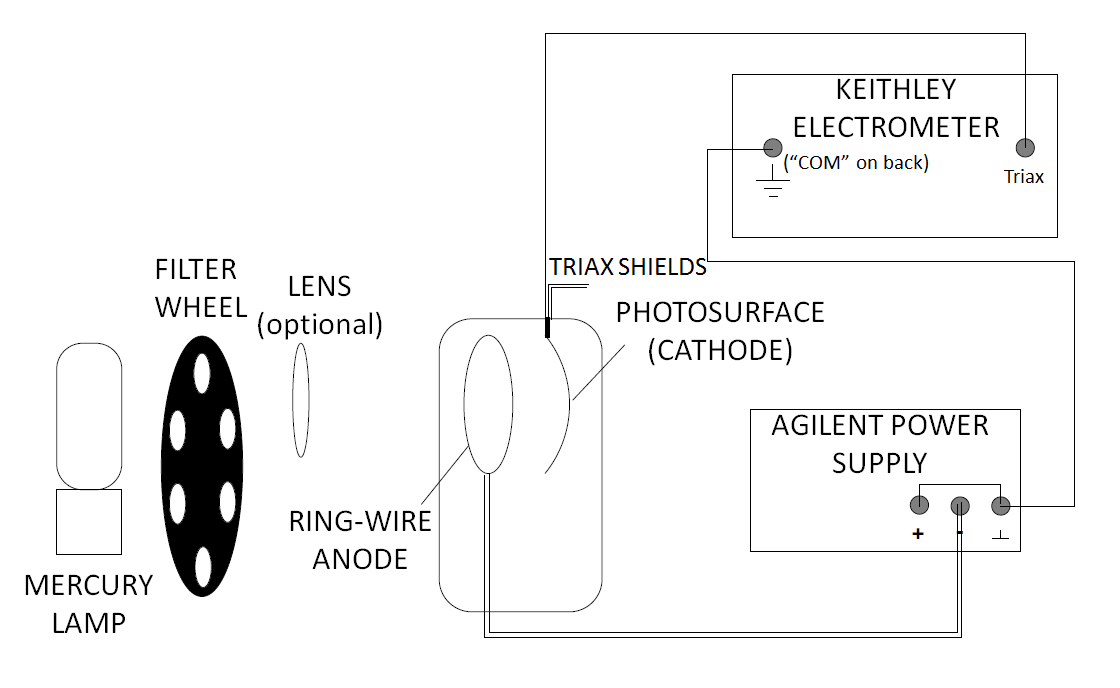
\includegraphics[width=10cm]{apparatus_setup.png}
	\caption{Signal chain for the photoelectric effect apparatus.}
\end{figure}
\end{frame}


%;;;;;;;;;;;;;;;;;;;;;;;;;;;;;;;;;;;;;;;;;;;;;;;;;;;;;;;;;;;;;;;;;;;;;;;;;;;;;;;;;;;;;
\begin{frame}{How Photocurrent Varies with Voltage and Filter}
 \begin{figure}
  \centering
  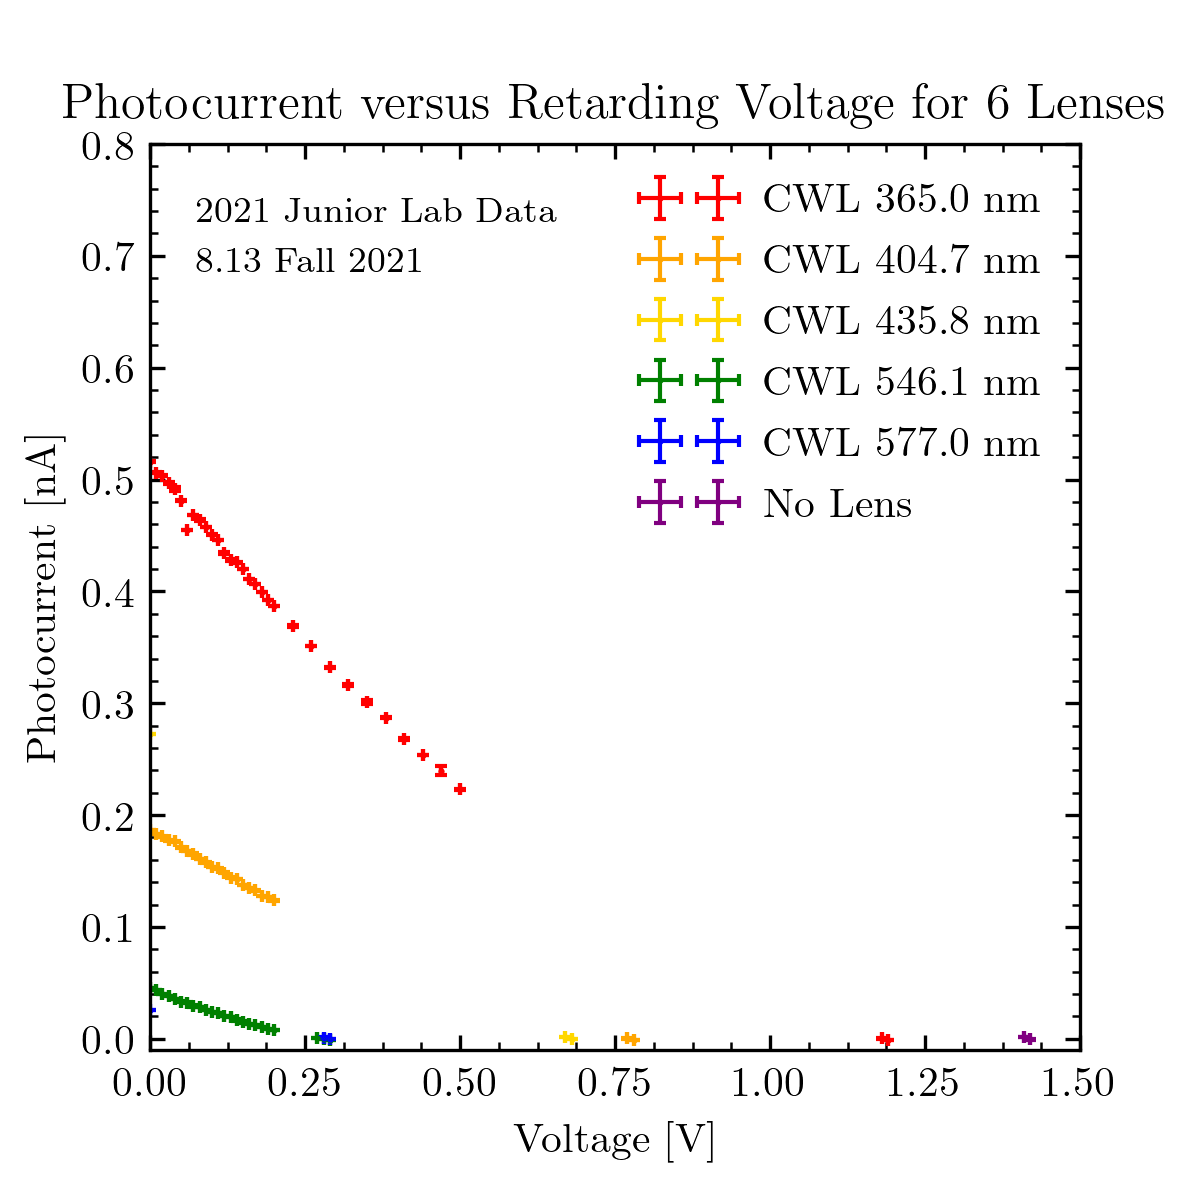
\includegraphics[height=7cm]{all_lenses_scatter.png}
  \caption{The photocurrent vs. retarding voltage relation for 6 filters. }
 \end{figure}
\end{frame}


%;;;;;;;;;;;;;;;;;;;;;;;;;;;;;;;;;;;;;;;;;;;;;;;;;;;;;;;;;;;;;;;;;;;;;;;;;;;;;;;;;;;;;
\begin{frame}{Variation of Photocurrent with Retarding Voltage}
\begin{figure}
	\centering
	\begin{minipage}{0.45\textwidth}
		\centering
		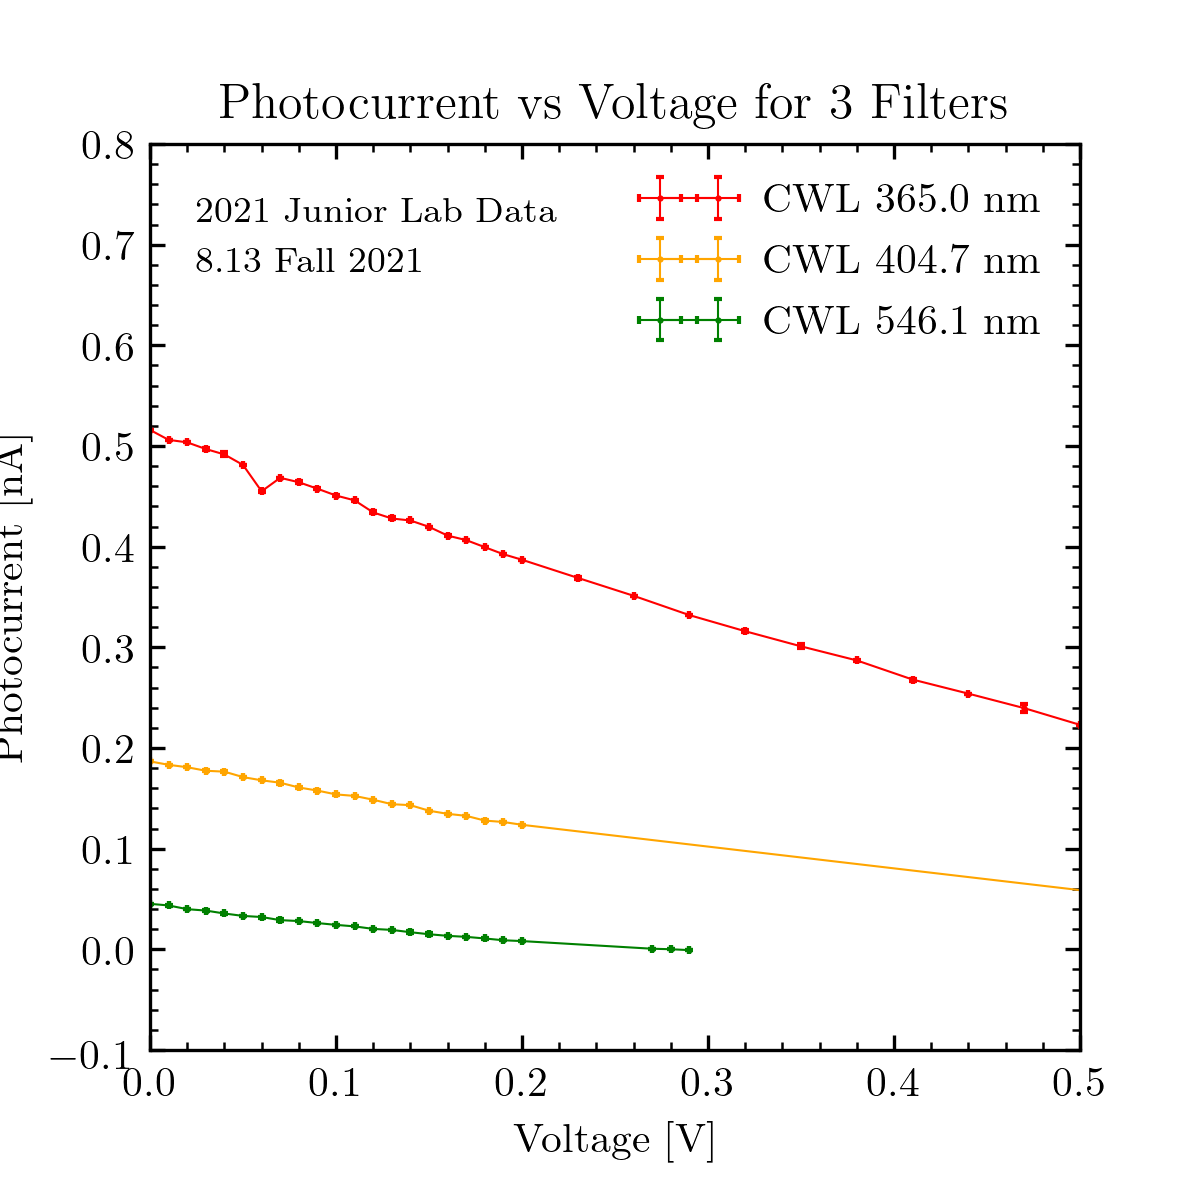
\includegraphics[width=1.1\textwidth]{4_lenses_scatter.png} % first figure itself
	\end{minipage}\vspace{0.55cm}
	\begin{minipage}{0.45\textwidth}
		\centering
		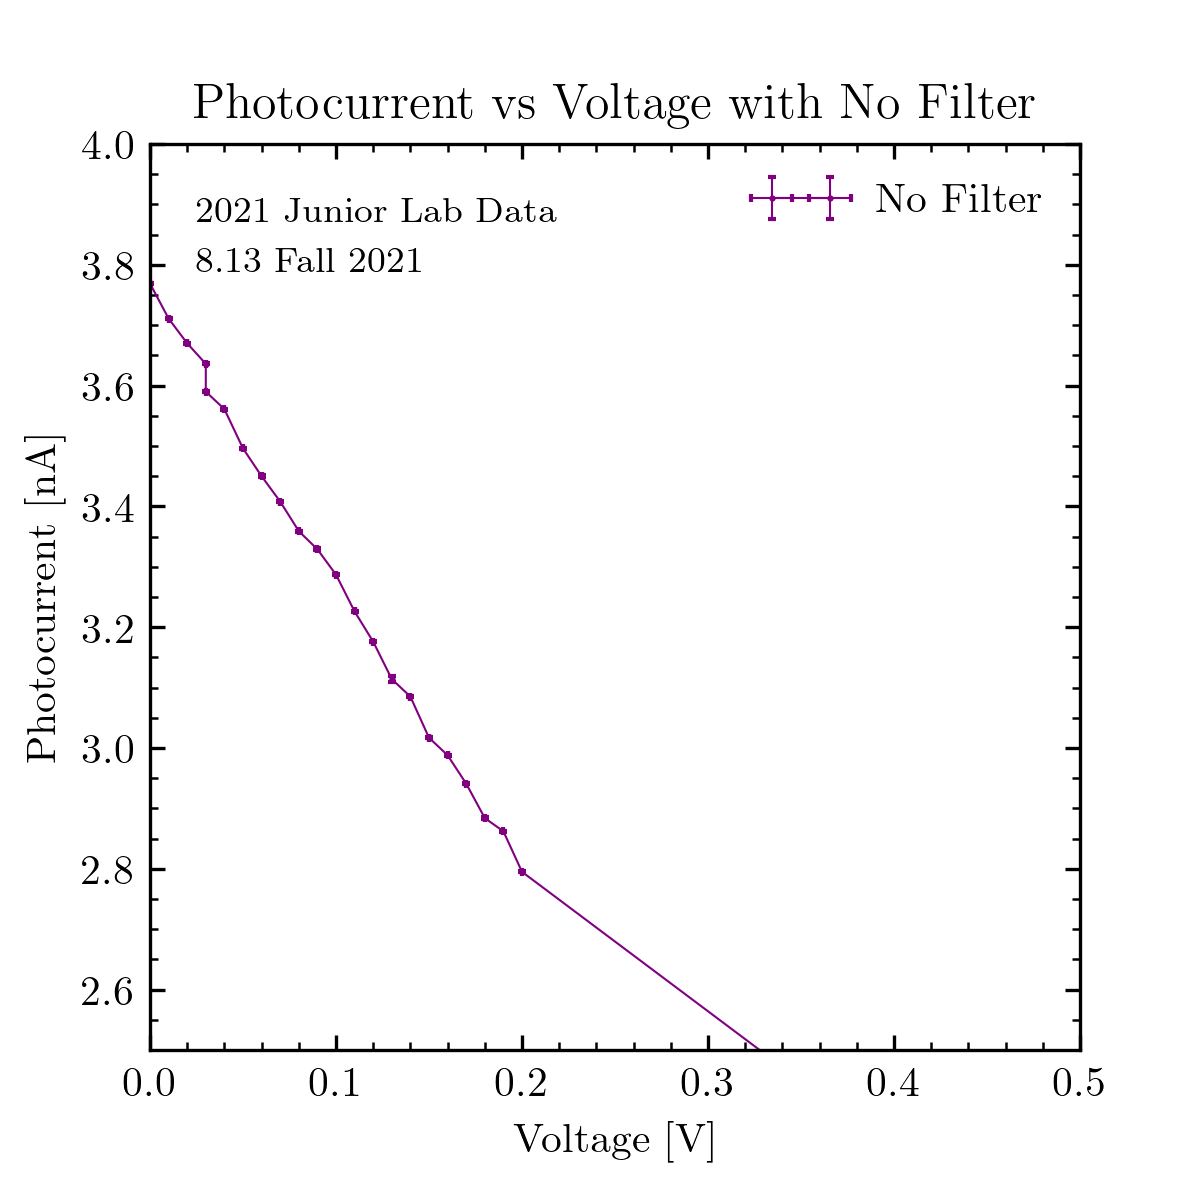
\includegraphics[width=1.1\textwidth]{nolens_scatter.png} % second figure itself
	\end{minipage}
\end{figure}
The left figure displays the photocurrent variation with retarding voltage across 3 different filters with different central wavelengths. The right figure displays the same plot but with no filter.
\end{frame}


\section{Extracting the Mean Velocity of Cosmic-Ray Muons}
\subsection{Determination of the mean slant path travel distance}

%;;;;;;;;;;;;;;;;;;;;;;;;;;;;;;;;;;;;;;;;;;;;;;;;;;;;;;;;;;;;;;;;;;;;;;;;;;;;;;;;;;;;;
\begin{frame}{\Large Stopping Voltage Vs. Incident Frequency}
 \begin{figure}
 	\centering
 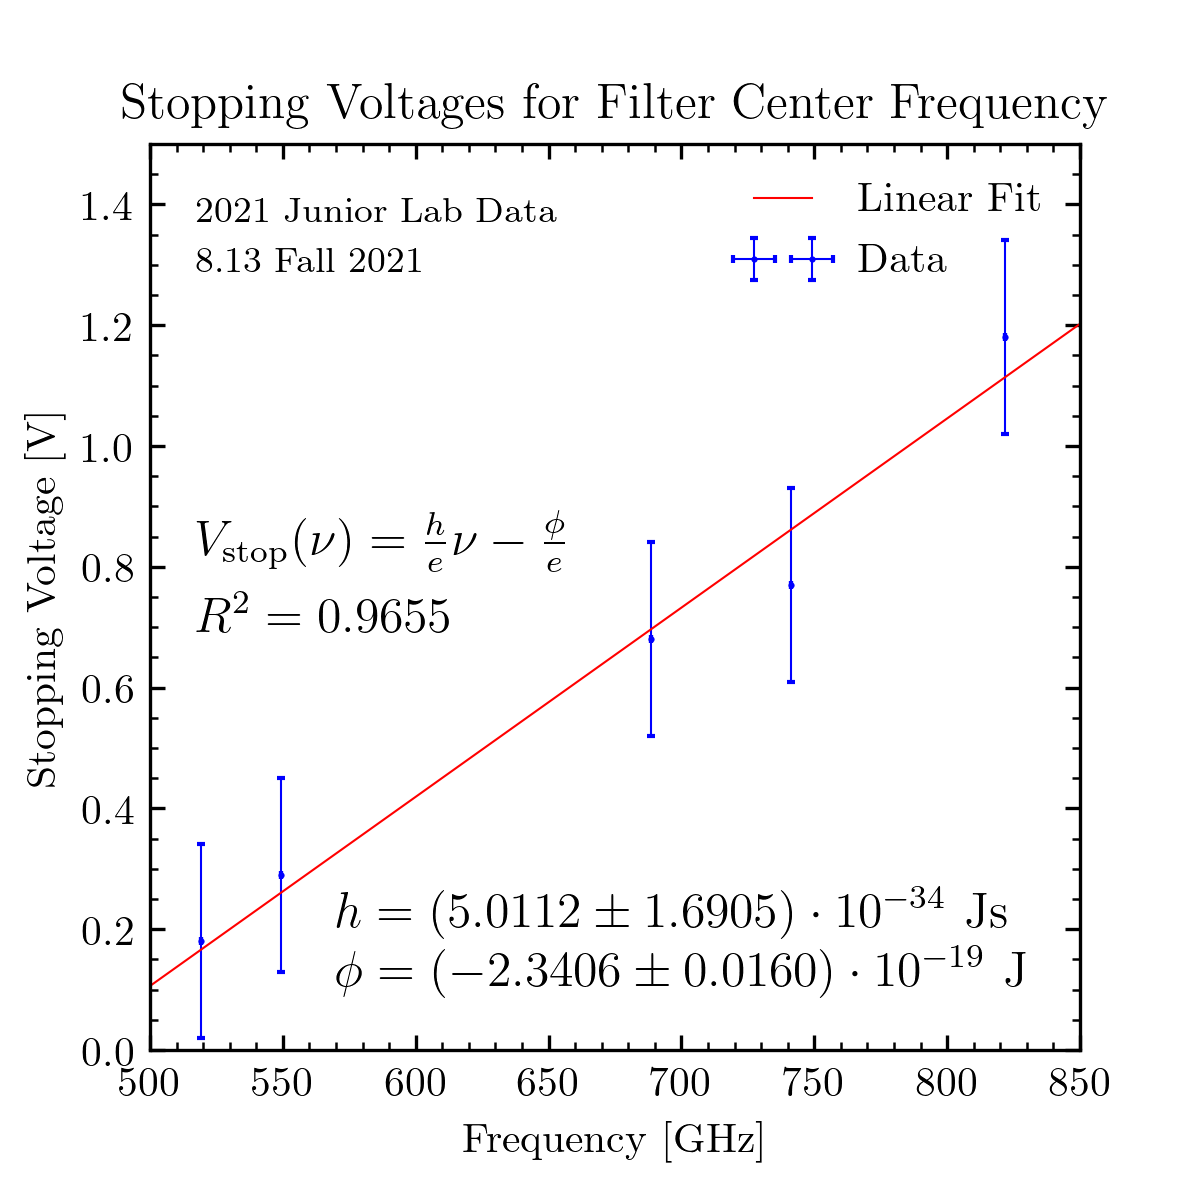
\includegraphics[height=7cm]{stopping_volts.png}
 \caption{A linear fit to the $V_{\mathrm{stop}}$ vs Frequency data, with stadard error bars. }
 \end{figure}
\end{frame}

%;;;;;;;;;;;;;;;;;;;;;;;;;;;;;;;;;;;;;;;;;;;;;;;;;;;;;;;;;;;;;;;;;;;;;;;;;;;;;;;;;;;;;
\begin{frame}{\Large Results and Interpretation}
\begin{itemize}
 \item For Planck's constant, I find a somewhat imprecise result: $$h = (5.0112\pm1.5302_{sys}\pm0.1603_{\mathrm{stat}})\cdot 10^{-34} J\cdot s$$
 \item Contributors to the systematic error: 
 \begin{itemize}
 	\item Missing calibration in the photocell $\rightarrow$ due to inhomogeneities in the metal surface, work function is not uniform. We did not always ensure that the same region was illuminated
 	\item distance from the mercury lamp to the photodiode was not recorded or kept constant.
 \end{itemize}
 \item Other sources of error:
 \begin{itemize}
	\item each frequency (i.e. filter) used, but generally only 1 trial for each. Contributed to higher standard error
	\item some fluctuations in the electrometer when measuring photocurrent leads to uncertainty of where they actual $V_{\mathrm{stop}}$ is.
	
  \end{itemize}
\end{itemize}
\end{frame}


%;;;;;;;;;;;;;;;;;;;;;;;;;;;;;;;;;;;;;;;;;;;;;;;;;;;;;;;;;;;;;;;;;;;;;;;;;;;;;;;;;;;;;
\begin{frame}{Summary and Conclusions}

  % Keep the summary *very short*.
\begin{itemize}
 \item We calculated Planck's constant $h$ to within 24\% of the known value
 \item We could have improved our experimental process by more stricty observing sources of systematic uncertainty; i.e. calibration
 \item We could also have budgeted our lab time to allow for more repeated data collection
 \item More broadly, we did oberse an increading stopping voltage with higher incident frequency, meaning that we accurately observed the behavior of the photoelectric effect. 
 \begin{itemize}
 	\item the increasing stopping voltage indicates that light waves do indeed behave as particles, in that greater energy is required to eject electrons against stronger retarding voltages
 \end{itemize}

\end{itemize}


\end{frame}



%;;;;;;;;;;;;;;;;;;;;;;;;;;;;;;;;;;;;;;;;;;;;;;;;;;;;;;;;;;;;;;;;;;;;;;;;;;;;;;;;;;;;;
% If you are using the verbatim environment make the frame [fragile]
%\begin{frame}[fragile]
%\frametitle {\bf {\Large Creating Slide Presentations in \LaTeX} }

%{\small As you can see, \LaTeX \ can be used to create very nice
%looking frames. \LaTeX \ Takes care of much of the formatting
%automatically when you use the ``frames'' environment.  Here's an
%example of what you should include at the beginning of your
%document:}%\pause


%{\tiny
%\begin{quote}  % Using quote environment for indentation
%\begin{verbatim}
%\documentclass{beamer}
%\usepackage{graphicx}
%\usepackage{graphics}
%\pagestyle{empty} \special{landscape} \special{! /landplus90 true
%store}

%\begin{document}
%...
%\end{verbatim}
%\end{quote}%\pause
% These commands tell it to add packages needed to incorporate graphics,
%  suppress page numbering and begin the document.  The
% ``special'' commands are hints to dvips which tell it to properly
% output a landscape format postscript file; the {\tt landplus90} bit
% fixes a bug in dvips which results in upside-down landscape format
% files.


%See the comments in the code for this document for more details on
%these commands.  Each frame is bounded by the frame environment:
%\pause
%\begin{quote}
%\begin{verbatim}
%\begin{frame}
%...
%\end{verbatim}
%\end{quote}
%}

%\end{frame}



\end{document}
